\chapter{Background} \label{c:Background}
This chapter will provide the necessary background in continuum mechanics and mathematics in order to understand the next chapters.

In this chapter we will examine the topic of the paper \textit{Stable Neo-Hookean Flesh Simulation}. The goal of the paper was to model deformations for virtual characters that have human-like features.


\section{Notation and Convention}

\subsection{General Notation}
At first we will declare the notation used in this thesis to avoid misunderstandings. We will use the common notation used in continuum mechanics and additionally we will include the declarations in the paper \textit{Stable Neo-Hookean Flesh Simulation}. 
\\
Scalars are represented by regular, normal-weight variables whereas 
tensors and matrices are represented by upper-case bold letters. Vectors will be denoted by bold lower-case variables.


\subsection{Tensor Notation}

Furthermore we will use the tensor notation used in the paper \textit{Stable Neo-Hookean Flesh Simulation}. They decided to to define vectorization vec(.) as column-wise flattening of a matrix into a vector (\cite{Smith:2018:SNF:3191713.3180491}, 12:5) similar to Golub and Van Loan (2012):

\[
\textbf{A} = \begin{bmatrix} a & c \\ b & d \end{bmatrix} \qquad vec(\textbf{A}) = \boldsymbol{\check{a}} = \begin{bmatrix} a \\ b \\ c \\ d \end{bmatrix}.
\]

In order to indicate that we are dealing with a vectorized matrix we will use the symbol $\check{.}$ as shown above.

Additionally we well have to deal with $4^{th}$ order tensors in the following matrix-of-matrices form:

\[
\mathbb{A} = 
\left[\begin{array}{cc}{\begin{bmatrix} a & c \\ b & d \end{bmatrix}} & {\begin{bmatrix} a & c \\ b & d \end{bmatrix}} \\ {\begin{bmatrix} a & c \\ b & d \end{bmatrix}} & {\begin{bmatrix} a & c \\ b & d \end{bmatrix}}\end{array}\right]
=
\left[\begin{array}{cc}{\left[\mathbf{A}_{00}\right]} & {\left[\mathbf{A}_{01}\right]} \\ {\left[\mathbf{A}_{10}\right]} & {\left[\mathbf{A}_{11}\right]}\end{array}\right]
\]

These matrices are denoted by using blackboard bold.

TODO: 2nd order matrix, see paper 4.1 Tensor Notation

\subsection{Summary}
A quick overview of the used notation:

\begin{addmargin}[2cm]{2cm}
a: scalar \\
\textbf{A}: matrix or tensor \\
\textbf{a}: vector \\
vec(\textbf{A}) = $\boldsymbol{\check{a}}$: vectorized matrix \\
\end{addmargin}

\section{Mathematical Background}

Since mathematics plays an important role in our field of interest we will build a solid background in this chapter. A basic understanding of linear algebra is assumed.

\subsection{Matrices}
At first we will discuss the geometrical meaning of some common matrix properties.


\subsection{Singular Value Decomposition}

The singular value decomposition (SVD) will play an important role in the following. It is important for our application since it represents the best possible approximation of a given matrix by a matrix of low rank. This approximation can be looked at as a compression of the data given (\cite{LiesenMehrmann2015}, S. 295).

\section{Continuum Mechanics}
In this section we will give a broad introduction the field of Continuum Mechanics.
In Continuum Mechanics we are less interested in small particles like atoms or molecules of an object but concentrate on pieces of matter which are in comparison very large. We are therefore concerned with the mechanical behavior of solids and fluids on the macroscopic scale (\cite{Spencer1980}, S. 1).


\section{Deformation}
Graphically we can imagine a deformation with the help of a deformation map. In Fig. \ref{fig:deformationmap} we have on the left side an ellipse that signifies an object in its rest state. On the right side in the same image we can see the ellipse in a deformed state. We can map each point from its rest state to the deformed one with the help of the function $\phi$.

\begin{figure}[!htbp]
	\centering
	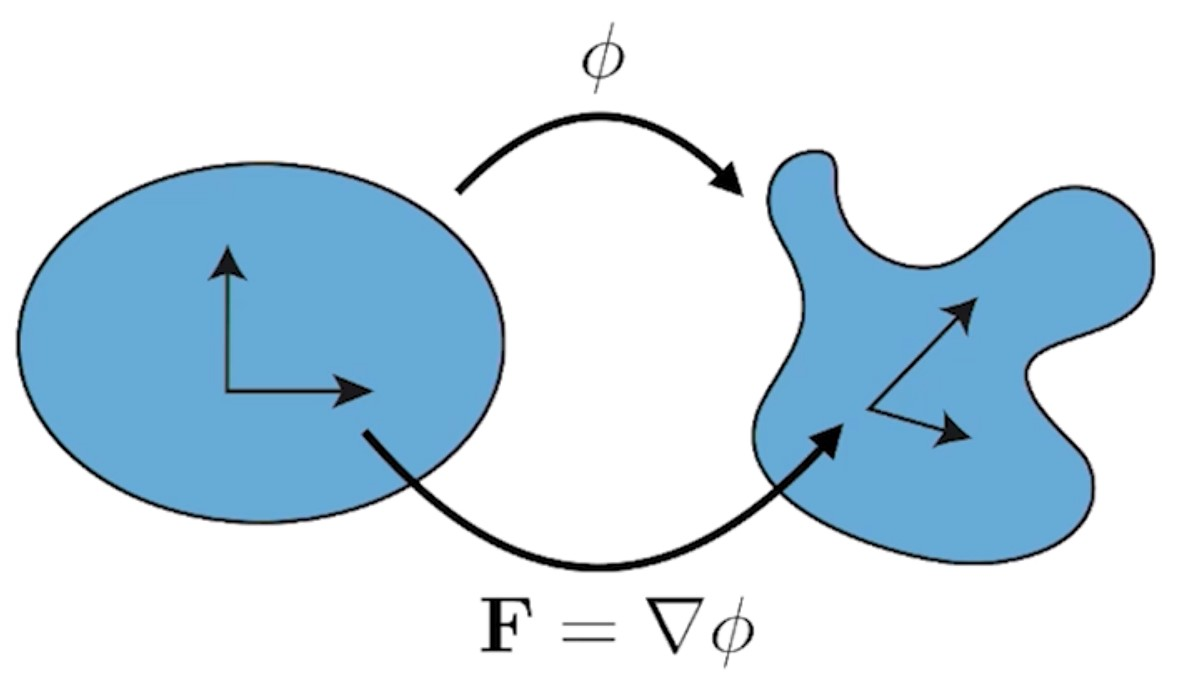
\includegraphics[width=0.5\textwidth]{resources/deformation_map}
	\caption{Deformation Map {\cite{STREAM2018}}}
	\label{fig:deformationmap}
\end{figure}

When applying a force over an object naturally the object itself undergoes a deformation. In the following we will be consistent with most previous literature in continuum mechanics and use the term strain as a measure of deformation and stress as the force per unit area.

\begin{addmargin}[2cm]{2cm}
\textit{Strain = measure of deformation}  \\
\textit{Stress = force per unit area} 
\end{addmargin}


\section{Deformation Gradient}

The deformation gradient $F$ is also shown in Fig. \ref{fig:deformationmap}. It offers us a measurement of the deformation. With its help we can amongst other things calculate the volume and length change an object undergoes during a deformation.
For our needs we define the deformation gradient as followed:

\[
\textbf{F} = \left[ \,f_0\, \bigg| \,f_1\, \bigg| \,f_2\, \right] = \begin{bmatrix} f_0 & f_3 & f_6 \\ f_1 & f_4 & f_7 \\ f_2 & f_5 & f_8 \end{bmatrix}
\]


Measure for the deformation, length and volume change etc.
Nonlinear deformations
http://www.continuummechanics.org/deformationgradient.html
also add some examples

\section{Material Constants}

Naturally the properties of the material the object consists of play an important rule in the deformation process. The two constants $\mu$ and $\lambda$ that are crucial for us are called \textit{Lamé Parameters}. The formula in which they appear is called \textit{Poisso's Ratio} and is of the following form:

\[ \sigma =  \frac{\lambda}{2(\lambda + \mu)} \in [-1, 0.5] \]

The poisson's ratio is of importance for us since it characterizes the materials resistance to volume change. Usually the poisson's ratio of a material is positive.
\\
For the simulation of human-like flesh we have to choose a poisson's ratio that is almost 0.5 to get realistic results.
\\ further reading: http://silver.neep.wisc.edu/~lakes/PoissonIntro.html


\section{Deformation Energy}

In order to get a convincing simulation of high quality we must choose an appropriate energy. In the case of modelling deformations on human-like characters we have to choose an elastic energy. The key property that makes an energy elastic is that if all the forces that are applied over an object add up to zero the object must come back to its rest shape.
\\
The energy then has to be minimized to get the results we want.

\begin{definition}
  This is a definition.
\end{definition}



